\documentclass{article}
\usepackage{color}
\usepackage{amsmath}
\usepackage{float}
\usepackage{tikz}
\usepackage{pgfplots}
\pgfplotsset{compat=1.18}
\usepackage[margin=1in]{geometry}
\definecolor{Othertext}{RGB}{51,51,51}
\title{\color{Othertext}Matrix Analysis Report}
\author{\color{Othertext}Generated by Matrix Class}
\begin{document}
\date{\color{Othertext}\today}
\maketitle


\section{Original Matrix}
\[
\begin{bmatrix}
-1.0000 & 2.0000 & 3.0000 & 4.0000 & 5.0000 \\
6.0000 & 7.0000 & 8.0000 & 9.0000 & 10.0000 \\
11.0000 & 12.1000 & 13.4000 & 14.4000 & 15.8000 \\
16.9000 & 17.8000 & 18.0000 & 19.7000 & 20.6000 \\
21.3000 & 22.2000 & 23.6000 & 24.1000 & 25.0000
\end{bmatrix}
\]

\section{Determinant}
The determinant of the matrix is:
\[
det(A) = -17.340\]

\section{Trace}
The trace of the matrix is:
\[
Tr(A) = 64.100\]

\section{Inverse Matrix}
The inverse of the matrix is:
\[
\begin{bmatrix}
-0.5052 & 0.7093 & -0.0346 & -0.0692 & -0.1038 \\
0.8069 & -3.8791 & 2.0461 & 0.7589 & -0.5283 \\
-0.0076 & 0.3070 & -0.0507 & -0.9348 & 0.6811 \\
-0.3640 & 6.3486 & -5.7601 & 0.1465 & 1.0530 \\
0.0720 & -3.5696 & 3.8132 & 0.1263 & -1.0606
\end{bmatrix}
\]

\section{Verification}
Multiplying the original matrix with its inverse ($A \cdot A^{-1}$) should give the identity matrix:
\[
\begin{bmatrix}
1.0000 & -0.0000 & 0.0000 & 0.0000 & -0.0000 \\
0.0000 & 1.0000 & 0.0000 & -0.0000 & -0.0000 \\
0.0000 & -0.0000 & 1.0000 & -0.0000 & -0.0000 \\
0.0000 & 0.0000 & -0.0000 & 1.0000 & -0.0000 \\
0.0000 & -0.0001 & 0.0000 & -0.0001 & 1.0000
\end{bmatrix}
\]

\section{Eigenvalues}
The eigenvalues of the matrix are:
\[
\begin{aligned}
\lambda_1 &= 69.776 \\
\lambda_2 &= -5.150 \\
\lambda_3 &= -0.768 \\
\lambda_4 &= 0.400 \\
\lambda_5 &= -0.157
\end{aligned}
\]
\section{Matrix Norms}
\begin{align*}
\text{Frobenius Norm} &= 75.744\\
\text{Maximum Norm} &= 25.000
\end{align*}

\section{Matrix Properties}
\begin{itemize}
\item Symmetric: No
\item Orthogonal: No
\item Positive Definite: No
\item Rank: 5 (Nullity: 0)
\end{itemize}

\section{Statistical Analysis}
\subsection{Basic Statistics}
\begin{align*}
\text{Mean} &= 13.156\\
\text{Variance} &= 56.406\\
\text{Sum} &= 328.900
\end{align*}

\section{Matrix Decompositions}
\subsection{LU Decomposition}
\[L
 = \begin{bmatrix}
1.0000 & 0.0000 & 0.0000 & 0.0000 & 0.0000 \\
-6.0000 & 1.0000 & 0.0000 & 0.0000 & 0.0000 \\
-11.0000 & 1.7947 & 1.0000 & 0.0000 & 0.0000 \\
-16.9000 & 2.7158 & 7.2601 & 1.0000 & 0.0000 \\
-21.3000 & 3.4105 & 4.4601 & 0.1191 & 1.0000
\end{bmatrix}
\]

\[U
 = \begin{bmatrix}
-1.0000 & 2.0000 & 3.0000 & 4.0000 & 5.0000 \\
0.0000 & 19.0000 & 26.0000 & 33.0000 & 40.0000 \\
0.0000 & 0.0000 & -0.2632 & -0.8263 & -0.9895 \\
0.0000 & 0.0000 & -0.0000 & 3.6781 & 3.6521 \\
0.0000 & -0.0000 & 0.0000 & 0.0000 & -0.9429
\end{bmatrix}
\]

\section{Matrix Visualization}
\subsection{Heatmap}
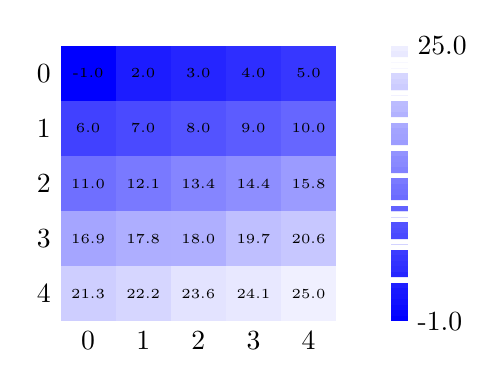
\begin{tikzpicture}[scale=0.7]
\definecolor{minColor}{RGB}{240,240,255}
\definecolor{maxColor}{RGB}{0,0,255}
\fill[minColor!0!maxColor] (0,4) rectangle (1,5);
\node at (0.5,4.5) {\tiny -1.0};
\fill[minColor!11.5!maxColor] (1.0,4.0) rectangle (2.0,5.0);
\node at (1.5,4.5) {\tiny 2.0};
\fill[minColor!15.4!maxColor] (2.0,4.0) rectangle (3.0,5.0);
\node at (2.5,4.5) {\tiny 3.0};
\fill[minColor!19.2!maxColor] (3.0,4.0) rectangle (4.0,5.0);
\node at (3.5,4.5) {\tiny 4.0};
\fill[minColor!23.1!maxColor] (4.0,4.0) rectangle (5.0,5.0);
\node at (4.5,4.5) {\tiny 5.0};
\fill[minColor!26.9!maxColor] (0.0,3.0) rectangle (1.0,4.0);
\node at (0.5,3.5) {\tiny 6.0};
\fill[minColor!30.8!maxColor] (1.0,3.0) rectangle (2.0,4.0);
\node at (1.5,3.5) {\tiny 7.0};
\fill[minColor!34.6!maxColor] (2.0,3.0) rectangle (3.0,4.0);
\node at (2.5,3.5) {\tiny 8.0};
\fill[minColor!38.5!maxColor] (3.0,3.0) rectangle (4.0,4.0);
\node at (3.5,3.5) {\tiny 9.0};
\fill[minColor!42.3!maxColor] (4.0,3.0) rectangle (5.0,4.0);
\node at (4.5,3.5) {\tiny 10.0};
\fill[minColor!46.2!maxColor] (0.0,2.0) rectangle (1.0,3.0);
\node at (0.5,2.5) {\tiny 11.0};
\fill[minColor!50.4!maxColor] (1.0,2.0) rectangle (2.0,3.0);
\node at (1.5,2.5) {\tiny 12.1};
\fill[minColor!55.4!maxColor] (2.0,2.0) rectangle (3.0,3.0);
\node at (2.5,2.5) {\tiny 13.4};
\fill[minColor!59.2!maxColor] (3.0,2.0) rectangle (4.0,3.0);
\node at (3.5,2.5) {\tiny 14.4};
\fill[minColor!64.6!maxColor] (4.0,2.0) rectangle (5.0,3.0);
\node at (4.5,2.5) {\tiny 15.8};
\fill[minColor!68.8!maxColor] (0.0,1.0) rectangle (1.0,2.0);
\node at (0.5,1.5) {\tiny 16.9};
\fill[minColor!72.3!maxColor] (1.0,1.0) rectangle (2.0,2.0);
\node at (1.5,1.5) {\tiny 17.8};
\fill[minColor!73.1!maxColor] (2.0,1.0) rectangle (3.0,2.0);
\node at (2.5,1.5) {\tiny 18.0};
\fill[minColor!79.6!maxColor] (3.0,1.0) rectangle (4.0,2.0);
\node at (3.5,1.5) {\tiny 19.7};
\fill[minColor!83.1!maxColor] (4.0,1.0) rectangle (5.0,2.0);
\node at (4.5,1.5) {\tiny 20.6};
\fill[minColor!85.8!maxColor] (0.0,0.0) rectangle (1.0,1.0);
\node at (0.5,0.5) {\tiny 21.3};
\fill[minColor!89.2!maxColor] (1.0,0.0) rectangle (2.0,1.0);
\node at (1.5,0.5) {\tiny 22.2};
\fill[minColor!94.6!maxColor] (2.0,0.0) rectangle (3.0,1.0);
\node at (2.5,0.5) {\tiny 23.6};
\fill[minColor!96.5!maxColor] (3.0,0.0) rectangle (4.0,1.0);
\node at (3.5,0.5) {\tiny 24.1};
\fill[minColor!100.0!maxColor] (4.0,0.0) rectangle (5.0,1.0);
\node at (4.5,0.5) {\tiny 25.0};
\node[left] at (0,4.5) {0};
\node[left] at (0,3.5) {1};
\node[left] at (0,2.5) {2};
\node[left] at (0,1.5) {3};
\node[left] at (0,0.5) {4};
\node[below] at (0.5,0) {0};
\node[below] at (1.5,0) {1};
\node[below] at (2.5,0) {2};
\node[below] at (3.5,0) {3};
\node[below] at (4.5,0) {4};
\fill[minColor!0!maxColor] (6.0,0.0) rectangle (6.3,0.1);
\fill[minColor!1!maxColor] (6.0,0.1) rectangle (6.3,0.1);
\fill[minColor!2!maxColor] (6.0,0.1) rectangle (6.3,0.2);
\fill[minColor!3!maxColor] (6.0,0.2) rectangle (6.3,0.2);
\fill[minColor!4!maxColor] (6.0,0.2) rectangle (6.3,0.3);
\fill[minColor!5!maxColor] (6.0,0.2) rectangle (6.3,0.3);
\fill[minColor!6!maxColor] (6.0,0.3) rectangle (6.3,0.4);
\fill[minColor!7!maxColor] (6.0,0.3) rectangle (6.3,0.4);
\fill[minColor!8!maxColor] (6.0,0.4) rectangle (6.3,0.5);
\fill[minColor!9!maxColor] (6.0,0.4) rectangle (6.3,0.5);
\fill[minColor!10!maxColor] (6.0,0.5) rectangle (6.3,0.6);
\fill[minColor!11!maxColor] (6.0,0.6) rectangle (6.3,0.6);
\fill[minColor!12!maxColor] (6.0,0.6) rectangle (6.3,0.7);
\fill[minColor!13!maxColor] (6.0,0.6) rectangle (6.3,0.7);
\fill[minColor!14!maxColor] (6.0,0.7) rectangle (6.3,0.7);
\fill[minColor!15!maxColor] (6.0,0.8) rectangle (6.3,0.8);
\fill[minColor!16!maxColor] (6.0,0.8) rectangle (6.3,0.9);
\fill[minColor!17!maxColor] (6.0,0.9) rectangle (6.3,0.9);
\fill[minColor!18!maxColor] (6.0,0.9) rectangle (6.3,0.9);
\fill[minColor!19!maxColor] (6.0,0.9) rectangle (6.3,1.0);
\fill[minColor!20!maxColor] (6.0,1.0) rectangle (6.3,1.1);
\fill[minColor!21!maxColor] (6.0,1.0) rectangle (6.3,1.1);
\fill[minColor!22!maxColor] (6.0,1.1) rectangle (6.3,1.2);
\fill[minColor!23!maxColor] (6.0,1.1) rectangle (6.3,1.2);
\fill[minColor!24!maxColor] (6.0,1.2) rectangle (6.3,1.3);
\fill[minColor!25!maxColor] (6.0,1.2) rectangle (6.3,1.3);
\fill[minColor!26!maxColor] (6.0,1.3) rectangle (6.3,1.3);
\fill[minColor!27!maxColor] (6.0,1.4) rectangle (6.3,1.4);
\fill[minColor!28!maxColor] (6.0,1.4) rectangle (6.3,1.4);
\fill[minColor!29!maxColor] (6.0,1.5) rectangle (6.3,1.5);
\fill[minColor!30!maxColor] (6.0,1.5) rectangle (6.3,1.6);
\fill[minColor!31!maxColor] (6.0,1.5) rectangle (6.3,1.6);
\fill[minColor!32!maxColor] (6.0,1.6) rectangle (6.3,1.7);
\fill[minColor!33!maxColor] (6.0,1.6) rectangle (6.3,1.7);
\fill[minColor!34!maxColor] (6.0,1.7) rectangle (6.3,1.8);
\fill[minColor!35!maxColor] (6.0,1.8) rectangle (6.3,1.8);
\fill[minColor!36!maxColor] (6.0,1.8) rectangle (6.3,1.8);
\fill[minColor!37!maxColor] (6.0,1.9) rectangle (6.3,1.9);
\fill[minColor!38!maxColor] (6.0,1.9) rectangle (6.3,1.9);
\fill[minColor!39!maxColor] (6.0,2.0) rectangle (6.3,2.0);
\fill[minColor!40!maxColor] (6.0,2.0) rectangle (6.3,2.0);
\fill[minColor!41!maxColor] (6.0,2.0) rectangle (6.3,2.1);
\fill[minColor!42!maxColor] (6.0,2.1) rectangle (6.3,2.1);
\fill[minColor!43!maxColor] (6.0,2.2) rectangle (6.3,2.2);
\fill[minColor!44!maxColor] (6.0,2.2) rectangle (6.3,2.3);
\fill[minColor!45!maxColor] (6.0,2.2) rectangle (6.3,2.3);
\fill[minColor!46!maxColor] (6.0,2.3) rectangle (6.3,2.3);
\fill[minColor!47!maxColor] (6.0,2.3) rectangle (6.3,2.4);
\fill[minColor!48!maxColor] (6.0,2.4) rectangle (6.3,2.5);
\fill[minColor!49!maxColor] (6.0,2.5) rectangle (6.3,2.5);
\fill[minColor!50!maxColor] (6.0,2.5) rectangle (6.3,2.5);
\fill[minColor!51!maxColor] (6.0,2.5) rectangle (6.3,2.6);
\fill[minColor!52!maxColor] (6.0,2.6) rectangle (6.3,2.6);
\fill[minColor!53!maxColor] (6.0,2.7) rectangle (6.3,2.7);
\fill[minColor!54!maxColor] (6.0,2.7) rectangle (6.3,2.8);
\fill[minColor!55!maxColor] (6.0,2.8) rectangle (6.3,2.8);
\fill[minColor!56!maxColor] (6.0,2.8) rectangle (6.3,2.8);
\fill[minColor!57!maxColor] (6.0,2.8) rectangle (6.3,2.9);
\fill[minColor!58!maxColor] (6.0,2.9) rectangle (6.3,3.0);
\fill[minColor!59!maxColor] (6.0,3.0) rectangle (6.3,3.0);
\fill[minColor!60!maxColor] (6.0,3.0) rectangle (6.3,3.0);
\fill[minColor!61!maxColor] (6.0,3.0) rectangle (6.3,3.1);
\fill[minColor!62!maxColor] (6.0,3.1) rectangle (6.3,3.1);
\fill[minColor!63!maxColor] (6.0,3.2) rectangle (6.3,3.2);
\fill[minColor!64!maxColor] (6.0,3.2) rectangle (6.3,3.3);
\fill[minColor!65!maxColor] (6.0,3.2) rectangle (6.3,3.3);
\fill[minColor!66!maxColor] (6.0,3.3) rectangle (6.3,3.3);
\fill[minColor!67!maxColor] (6.0,3.3) rectangle (6.3,3.4);
\fill[minColor!68!maxColor] (6.0,3.4) rectangle (6.3,3.5);
\fill[minColor!69!maxColor] (6.0,3.5) rectangle (6.3,3.5);
\fill[minColor!70!maxColor] (6.0,3.5) rectangle (6.3,3.5);
\fill[minColor!71!maxColor] (6.0,3.5) rectangle (6.3,3.6);
\fill[minColor!72!maxColor] (6.0,3.6) rectangle (6.3,3.6);
\fill[minColor!73!maxColor] (6.0,3.7) rectangle (6.3,3.7);
\fill[minColor!74!maxColor] (6.0,3.7) rectangle (6.3,3.8);
\fill[minColor!75!maxColor] (6.0,3.8) rectangle (6.3,3.8);
\fill[minColor!76!maxColor] (6.0,3.8) rectangle (6.3,3.8);
\fill[minColor!77!maxColor] (6.0,3.8) rectangle (6.3,3.9);
\fill[minColor!78!maxColor] (6.0,3.9) rectangle (6.3,4.0);
\fill[minColor!79!maxColor] (6.0,4.0) rectangle (6.3,4.0);
\fill[minColor!80!maxColor] (6.0,4.0) rectangle (6.3,4.0);
\fill[minColor!81!maxColor] (6.0,4.1) rectangle (6.3,4.1);
\fill[minColor!82!maxColor] (6.0,4.1) rectangle (6.3,4.1);
\fill[minColor!83!maxColor] (6.0,4.2) rectangle (6.3,4.2);
\fill[minColor!84!maxColor] (6.0,4.2) rectangle (6.3,4.2);
\fill[minColor!85!maxColor] (6.0,4.2) rectangle (6.3,4.3);
\fill[minColor!86!maxColor] (6.0,4.3) rectangle (6.3,4.4);
\fill[minColor!87!maxColor] (6.0,4.3) rectangle (6.3,4.4);
\fill[minColor!88!maxColor] (6.0,4.4) rectangle (6.3,4.5);
\fill[minColor!89!maxColor] (6.0,4.4) rectangle (6.3,4.5);
\fill[minColor!90!maxColor] (6.0,4.5) rectangle (6.3,4.5);
\fill[minColor!91!maxColor] (6.0,4.6) rectangle (6.3,4.6);
\fill[minColor!92!maxColor] (6.0,4.6) rectangle (6.3,4.6);
\fill[minColor!93!maxColor] (6.0,4.7) rectangle (6.3,4.7);
\fill[minColor!94!maxColor] (6.0,4.7) rectangle (6.3,4.7);
\fill[minColor!95!maxColor] (6.0,4.8) rectangle (6.3,4.8);
\fill[minColor!96!maxColor] (6.0,4.8) rectangle (6.3,4.9);
\fill[minColor!97!maxColor] (6.0,4.8) rectangle (6.3,4.9);
\fill[minColor!98!maxColor] (6.0,4.9) rectangle (6.3,5.0);
\fill[minColor!99!maxColor] (6.0,4.9) rectangle (6.3,5.0);
\node[right] at (6.3,5.0) {25.0};
\node[right] at (6.3,0) {-1.0};
\end{tikzpicture}

\subsection{Row Means Distribution}
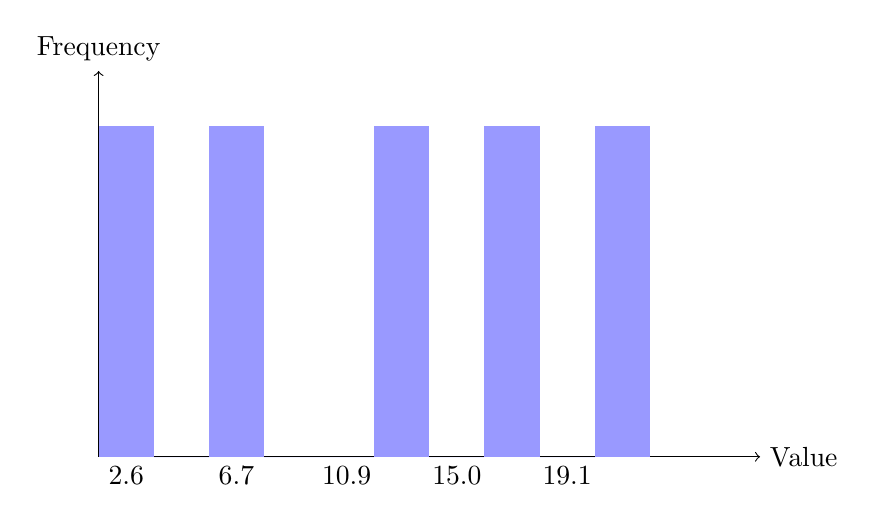
\begin{tikzpicture}[scale=0.7]
\draw[->] (0,0) -- (12,0) node[right] {Value};
\draw[->] (0,0) -- (0,7) node[above] {Frequency};
\fill[blue!40] (0,0) rectangle (1,6);
\node[below] at (0.5,0) {2.6};
\fill[blue!40] (1.0,0) rectangle (2.0,0.0);
\fill[blue!40] (2.0,0) rectangle (3.0,6.0);
\node[below] at (2.5,0) {6.7};
\fill[blue!40] (3.0,0) rectangle (4.0,0.0);
\fill[blue!40] (4.0,0) rectangle (5.0,0.0);
\node[below] at (4.5,0) {10.9};
\fill[blue!40] (5.0,0) rectangle (6.0,6.0);
\fill[blue!40] (6.0,0) rectangle (7.0,0.0);
\node[below] at (6.5,0) {15.0};
\fill[blue!40] (7.0,0) rectangle (8.0,6.0);
\fill[blue!40] (8.0,0) rectangle (9.0,0.0);
\node[below] at (8.5,0) {19.1};
\fill[blue!40] (9.0,0) rectangle (10.0,6.0);
\end{tikzpicture}

\end{document}
